\documentclass[aspectratio=169,10pt]{beamer}
\usepackage[T1]{fontenc}
\usepackage{amsmath,amssymb,amsfonts}
\usepackage{bm}
\usepackage{tikz}
\usepackage{xcolor}
\usetikzlibrary{arrows.meta,positioning,shapes,calc}

\definecolor{parchment}{HTML}{F4E8C8}
\definecolor{paper}{HTML}{FAF1D8}
\definecolor{ink}{HTML}{1A1A1A}
\definecolor{inkgray}{HTML}{5A5A5A}
\definecolor{accentred}{HTML}{8B1A1A}
\definecolor{accentgreen}{HTML}{2D5F2C}
\definecolor{accentblue}{HTML}{1F4E79}
\definecolor{redbg}{HTML}{F7E0DE}
\definecolor{grnbg}{HTML}{E0EBDC}
\definecolor{blubg}{HTML}{DDE6EF}
\definecolor{labelbg}{HTML}{EFE0B0}

\usefonttheme{serif}
\setbeamercolor{background canvas}{bg=parchment}
\setbeamercolor{normal text}{fg=ink}
\setbeamercolor{structure}{fg=ink}
\setbeamercolor{frametitle}{fg=ink,bg=parchment}
\setbeamercolor{title}{fg=ink}
\setbeamercolor{itemize item}{fg=ink}
\setbeamercolor{itemize subitem}{fg=ink}
\setbeamercolor{item}{fg=ink}
\setbeamercolor{caption name}{fg=ink}
\setbeamertemplate{navigation symbols}{}
\setbeamertemplate{itemize item}{\textbullet}

\setbeamertemplate{frametitle}{%
  \vspace{0.30em}%
  \begin{center}%
    {\bfseries\Large\insertframetitle\par}%
    \vspace{0.28em}%
    {\color{ink}\rule{0.86\paperwidth}{0.4pt}}%
  \end{center}%
  \vspace{0.10em}%
}
\setbeamertemplate{footline}{%
  \hbox to \paperwidth{\hfil\itshape\small\insertframenumber\hspace{0.7em}}%
  \vspace{0.35em}%
}

\newcommand{\vY}{\bm{Y}}
\newcommand{\vy}{\bm{y}}
\newcommand{\vA}{\bm{A}}
\newcommand{\vB}{\bm{B}}
\newcommand{\valpha}{\bm{\alpha}}
\newcommand{\vn}{\bm{n}}
\newcommand{\vs}{\bm{s}}
\newcommand{\vW}{\bm{W}}
\newcommand{\T}{^{\mathsf T}}
\newcommand{\Hh}{^{\mathsf H}}
\newcommand{\norm}[1]{\left\lVert #1\right\rVert}
\DeclareMathOperator*{\argmin}{arg\,min}

\tikzset{
  flowbox/.style={draw=ink,fill=paper,line width=0.6pt,
                  minimum width=2.5cm,minimum height=1.0cm,
                  align=center,font=\small\bfseries,inner sep=4pt},
  smallbox/.style={draw=ink,fill=paper,line width=0.4pt,
                   minimum width=0.7cm,minimum height=0.55cm,
                   inner sep=2pt,align=center,font=\footnotesize\itshape},
  method/.style={draw=accentgreen,fill=grnbg,line width=1.0pt,
                 align=center,font=\small\bfseries,inner sep=6pt},
  issue/.style={draw=accentred,fill=redbg,line width=1.0pt,
                align=center,font=\small\bfseries,inner sep=6pt},
  idea/.style={draw=accentblue,fill=blubg,line width=1.0pt,
               align=center,font=\small\bfseries,inner sep=6pt},
  flowarr/.style={-{Stealth[length=2.5mm,width=2mm]},line width=0.7pt},
  softarr/.style={-{Stealth[length=2mm,width=1.6mm]},line width=0.5pt,color=inkgray}
}

\newcommand{\bottomnote}[1]{%
  \begin{center}{\itshape\small #1}\end{center}}

\newcommand{\papercover}[4]{%
  \begin{frame}[plain]
    \vfill
    \begin{center}
      {\bfseries\Huge #1\par}
      \vspace{0.8cm}
      {\Large #2\par}
      \vspace{0.35cm}
      {\itshape\large\color{inkgray}#3\par}
      \vspace{0.55cm}
      {\small\texttt{\detokenize{#4}}\par}
    \end{center}
    \vfill
  \end{frame}}

\newcommand{\twocolmodel}[4]{%
  \begin{columns}[T,onlytextwidth]
    \begin{column}{0.48\textwidth}#1\end{column}
    \begin{column}{0.48\textwidth}#2\end{column}
  \end{columns}
  \bottomnote{#3\\#4}}


\usetikzlibrary{fit,decorations.pathreplacing}

\newcommand{\Kset}{\mathcal K}
\newcommand{\Pset}{\mathcal P}
\newcommand{\C}{\mathbb C}

\tikzset{
  card/.style={draw=ink,fill=paper,line width=0.55pt,rounded corners=2pt,
               align=center,inner sep=5pt,font=\small},
  goodcard/.style={draw=accentgreen,fill=grnbg,line width=0.85pt,
                   rounded corners=2pt,align=center,inner sep=5pt,font=\small},
  badcard/.style={draw=accentred,fill=redbg,line width=0.85pt,
                  rounded corners=2pt,align=center,inner sep=5pt,font=\small},
  bluecard/.style={draw=accentblue,fill=blubg,line width=0.85pt,
                   rounded corners=2pt,align=center,inner sep=5pt,font=\small},
  ghostcard/.style={draw=inkgray!65,fill=paper,line width=0.55pt,dashed,
                    rounded corners=2pt,align=center,inner sep=5pt,
                    font=\small,text=inkgray},
  vcell/.style={draw=ink,fill=paper,line width=0.55pt,
                minimum width=1.1cm,minimum height=0.6cm,
                inner sep=1pt,font=\small},
  pcell/.style={draw=ink,fill=paper,line width=0.4pt,
                minimum width=1.05cm,minimum height=0.58cm,
                inner sep=1pt,font=\scriptsize},
  redarr/.style={-{Stealth[length=2.5mm,width=2mm]},line width=0.85pt,
                  draw=accentred},
  greenarr/.style={-{Stealth[length=2.5mm,width=2mm]},line width=0.85pt,
                    draw=accentgreen},
  bluearr/.style={-{Stealth[length=2.5mm,width=2mm]},line width=0.85pt,
                   draw=accentblue},
  cpbrace/.style={decorate,decoration={brace,amplitude=5pt,raise=2pt},
                  line width=0.6pt,color=inkgray}
}

\begin{document}

% =====================================================================
% 1. Cover
% =====================================================================
\begin{frame}[plain]
  \centering
  \vspace{0.25cm}
  {\small\color{inkgray}Equation (10) of \texttt{juna\_joint\_ieee.tex}\par}
  \vspace{0.20cm}
  {\bfseries\Huge The Pilot-Trained Combiner\par}
  \vspace{0.25cm}
  {\Large One soft symbol from the $M$ partial-FFT views\par}
  \vspace{0.55cm}

  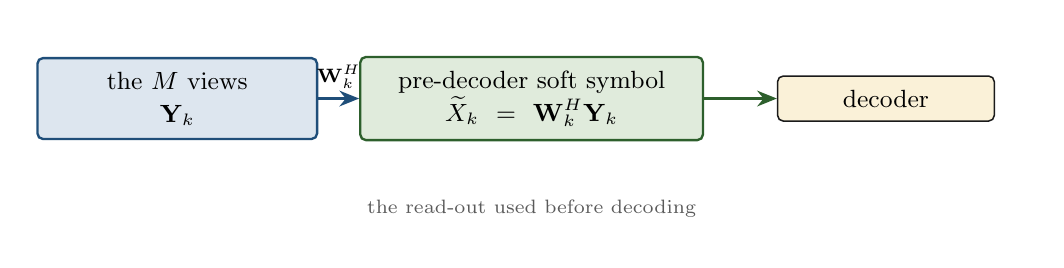
\begin{tikzpicture}[x=1cm,y=1cm]
    \path[use as bounding box] (-6.4,-1.5) rectangle (6.4,1.2);
    \node[bluecard,text width=3.2cm] (views) at (-4.5,0.3)
      {the $M$ views\\[0.1em]$\mathbf Y_k$};
    \node[goodcard,text width=4.0cm] (soft) at (0,0.3)
      {pre-decoder soft symbol\\[0.1em]
       $\widetilde X_k=\mathbf W_k^{H}\mathbf Y_k$};
    \node[card,text width=2.4cm] (dec) at (4.5,0.3) {decoder};
    \draw[bluearr] (views) -- (soft)
      node[midway,above,font=\scriptsize] {$\mathbf W_k^{H}$};
    \draw[greenarr] (soft) -- (dec);
    \node[font=\scriptsize\color{inkgray}] at (0,-1.1)
      {the read-out used before decoding};
  \end{tikzpicture}
\end{frame}

% =====================================================================
% 2. Partial-FFT views
% =====================================================================
\begin{frame}{Partial-FFT views}
  \centering
  \begin{tikzpicture}[x=1cm,y=1cm]
    \path[use as bounding box] (-6.5,-3.0) rectangle (6.5,2.5);

    \draw[->,line width=0.65pt] (-6.2,0.85) -- (0.9,0.85)
      node[right,font=\scriptsize] {time};

    \foreach \m/\xa in {1/-5.9,2/-4.4,3/-2.9,4/-1.4}{
      \draw[fill=blubg,draw=accentblue,line width=0.8pt]
        (\xa,1.10) rectangle ({\xa+1.5},1.90);
      \node[font=\small] at ({\xa+0.75},1.50) {$\mathcal T_{\m}$};
    }
    \node[font=\scriptsize\color{inkgray}] at (-3.15,2.22)
      {one OFDM symbol, $M=4$ windowed pieces};

    \only<2->{
      \foreach \m/\yc in {1/1.05,2/0.40,3/-0.25,4/-0.90}{
        \pgfmathsetmacro{\xs}{-5.15+1.5*(\m-1)}
        \draw[bluearr] (\xs,1.05)
          .. controls (\xs,\yc) and (2.2,\yc) .. (3.05,\yc);
        \node[vcell] at (3.75,\yc) {$Y_{k,\m}$};
      }
      \node[font=\scriptsize,align=center] at (-1.6,-1.95)
        {FFT of each windowed piece,\\taken at bin $k$};
    }

    \only<3->{
      \draw[cpbrace] (4.45,1.40) -- (4.45,-1.25);
      \node[font=\small,anchor=west] at (4.95,0.08) {$\mathbf Y_k$};
    }

    \only<4->{
      \node[bluecard,text width=5.4cm] at (3.6,-2.45)
        {$\displaystyle\sum_{m=1}^{M}Y_{k,m}=Y_k^{\mathrm{full}}$\\[0.1em]
         \scriptsize the views sum to the full-FFT bin};
    }
  \end{tikzpicture}
  \bottomnote{$\mathbf Y_k$ collects the $M$ views of carrier $k$: the FFT
    of each windowed piece of the block, taken at bin $k$.}
\end{frame}

% =====================================================================
% 3. The read-out
% =====================================================================
\begin{frame}{The read-out}
  \centering
  \begin{tikzpicture}[x=1cm,y=1cm]
    \path[use as bounding box] (-6.6,-3.05) rectangle (6.6,2.3);

    \foreach \m/\yc in {1/1.68,2/1.03,3/0.38,4/-0.27}{
      \node[vcell] at (-0.4,\yc) {$Y_{k,\m}$};
    }
    \only<1>{
      \node[font=\scriptsize,align=center] at (-0.4,-1.05)
        {$\mathbf Y_k$ --- the $M$ views};
    }
    \only<2->{
      \draw[cpbrace] (0.35,2.01) -- (0.35,-0.60);
      \node[font=\scriptsize,anchor=west,align=left] at (0.80,0.70)
        {$\mathbf Y_k$\\the $M$ views};
    }

    \only<2->{
      \foreach \m/\xc in {1/-5.5,2/-4.4,3/-3.3,4/-2.2}{
        \node[vcell,fill=blubg] at (\xc,0.70) {$W_{k,\m}^{*}$};
      }
      \node[font=\scriptsize,align=center] at (-3.85,-0.15)
        {$\mathbf W_k^{H}$ --- one weight per view};
    }

    \only<3->{
      \node[font=\large] at (2.45,0.70) {$=$};
      \node[vcell,fill=grnbg,minimum width=1.2cm] at (3.45,0.70)
        {$\widetilde X_k$};
      \node[font=\scriptsize,align=center] at (3.45,-0.15)
        {one pre-decoder\\soft symbol};
    }

    \only<4->{
      \node[font=\small] at (0,-1.35)
        {$\displaystyle\widetilde X_k=\sum_{m=1}^{M}W_{k,m}^{*}\,Y_{k,m}$};
      \node[bluecard,text width=9.6cm] at (0,-2.45)
        {$\widetilde X_k=\mathbf W_k^{H}\mathbf Y_k$\\[0.15em]
         \scriptsize equation (10), where $\mathbf W_k\in\C^{M}$ collects
         the combiner weights for carrier $k$};
    }
  \end{tikzpicture}
  \bottomnote{The weights rotate and scale the views back toward the
    transmitted symbol, and the pilots supply the carriers where that
    symbol is known.}
\end{frame}

% =====================================================================
% 4. The arcs
% =====================================================================
\begin{frame}{The arcs}
  \centering
  \begin{tikzpicture}[x=1cm,y=1cm]
    \path[use as bounding box] (-6.6,-2.75) rectangle (6.6,2.35);

    \begin{scope}[shift={(-4.6,-0.15)}]
      \draw[inkgray!50,dashed] (0,0) circle (1.05);
      \foreach \m/\ang in {1/0,2/50,3/100,4/150}{
        \draw[bluearr] (0,0) -- (\ang:1.02);
        \node[font=\scriptsize\color{accentblue}] at (\ang:1.28) {$\m$};
      }
      \node[font=\scriptsize,align=center] at (0.1,-1.90)
        {the views of one carrier differ\\by their per-segment phases};
    \end{scope}

    \only<2->{
      \begin{scope}[shift={(-1.3,-1.15)}]
        \draw[bluearr] (0,0) -- (0.80,0);
        \draw[bluearr] (0.80,0) -- (1.31,0.61);
        \draw[bluearr] (1.31,0.61) -- (1.18,1.40);
        \draw[bluearr] (1.18,1.40) -- (0.48,1.80);
        \draw[redarr,line width=1.3pt] (0,0) -- (0.48,1.80);
        \node[font=\scriptsize\color{accentred},align=center]
          at (0.85,-0.90) {plain sum:\\the full-FFT scalar};
      \end{scope}
    }

    \only<3->{
      \begin{scope}[shift={(2.3,-0.05)}]
        \foreach \i in {0,1,2,3}{
          \draw[bluearr] ({0.8*\i},0.55) -- ({0.8*\i+0.78},0.55);
        }
        \draw[greenarr,line width=1.3pt] (0,0) -- (3.2,0);
        \node[font=\scriptsize\color{accentgreen},align=center]
          at (1.6,-0.80) {aligned sum:\\one complex weight\\per view realigns them};
      \end{scope}
    }
  \end{tikzpicture}
  \bottomnote{Residual Doppler fans the arcs of one carrier in phase, so
    their plain sum, the full-FFT scalar, is shorter than the aligned sum
    the views still admit.}
\end{frame}

% =====================================================================
% 5. The ridge criterion
% =====================================================================
\begin{frame}{The ridge criterion}
  \centering
  {\small Every pilot is a carrier whose transmitted symbol the receiver
   knows.\par}
  \vspace{0.10cm}
  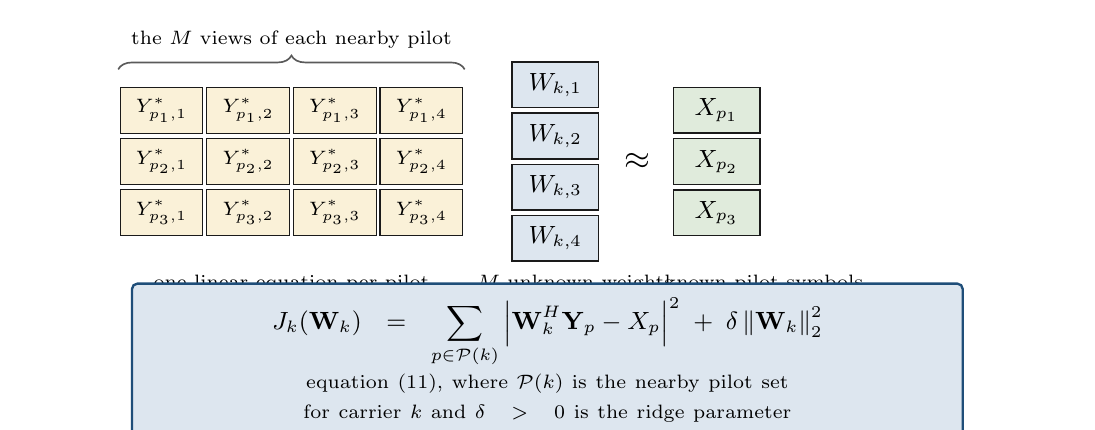
\begin{tikzpicture}[x=1cm,y=1cm]
    \path[use as bounding box] (-6.6,-2.85) rectangle (6.6,1.9);

    \foreach \p/\yc in {p_1/0.85,p_2/0.20,p_3/-0.45}{
      \foreach \m/\xc in {1/-4.9,2/-3.8,3/-2.7,4/-1.6}{
        \node[pcell] at (\xc,\yc) {$Y_{\p,\m}^{*}$};
      }
    }
    \draw[cpbrace] (-5.45,1.30) -- (-1.05,1.30);
    \node[font=\scriptsize] at (-3.25,1.75)
      {the $M$ views of each nearby pilot};
    \node[font=\scriptsize] at (-3.25,-1.35)
      {one linear equation per pilot};

    \foreach \m/\yc in {1/1.175,2/0.525,3/-0.125,4/-0.775}{
      \node[vcell,fill=blubg,minimum height=0.58cm] at (0.1,\yc)
        {$W_{k,\m}$};
    }
    \node[font=\scriptsize] at (0.35,-1.35) {$M$ unknown weights};

    \node[font=\large] at (1.15,0.20) {$\approx$};

    \foreach \p/\yc in {p_1/0.85,p_2/0.20,p_3/-0.45}{
      \node[vcell,fill=grnbg,minimum height=0.58cm] at (2.15,\yc)
        {$X_{\p}$};
    }
    \node[font=\scriptsize] at (2.75,-1.35) {known pilot symbols};

    \only<2->{
      \node[bluecard,text width=10.2cm] at (0,-2.32)
        {$\displaystyle J_k(\mathbf W_k)=\sum_{p\in\Pset(k)}
          \left|\mathbf W_k^{H}\mathbf Y_p-X_p\right|^2
          +\delta\left\lVert\mathbf W_k\right\rVert_2^2$\\[0.15em]
         \scriptsize equation (11), where $\Pset(k)$ is the nearby pilot
         set for carrier $k$ and $\delta>0$ is the ridge parameter};
    }
  \end{tikzpicture}
  \bottomnote{The nearby pilot set has to supply at least $M$ equations
    before the weights are determined, and the ridge keeps the fit stable
    when it supplies fewer.}
\end{frame}

% =====================================================================
% 6. The discard
% =====================================================================
\begin{frame}{The discard}
  \centering
  \begin{tikzpicture}[x=1cm,y=1cm]
    \path[use as bounding box] (-6.6,-2.85) rectangle (6.6,2.5);

    \foreach \m/\yc in {1/1.55,2/0.90,3/0.25,4/-0.40}{
      \node[vcell] at (-5.3,\yc) {$Y_{k,\m}$};
    }
    \node[font=\scriptsize] at (-5.3,2.05) {$\mathbf Y_k$};

    \node[goodcard,text width=2.0cm] (kept) at (-2.5,1.35)
      {$\mathbf W_k^{H}\mathbf Y_k$};
    \node[vcell,fill=grnbg,minimum width=1.2cm] (soft) at (0.4,1.35)
      {$\widetilde X_k$};
    \node[flowbox,fill=grnbg,draw=accentgreen] (dec) at (3.9,1.35)
      {decoder};
    \draw[greenarr] (-4.65,1.35) -- (kept.west);
    \draw[greenarr] (kept.east) -- (soft.west);
    \draw[greenarr] (soft.east) -- (dec.west);
    \node[font=\scriptsize\color{accentgreen},align=center] at (-1.0,2.20)
      {keeps one combination of a carrier's $M$ views};

    \only<2->{
      \node[ghostcard,text width=3.3cm] (rest) at (-2.2,-1.15)
        {the other $M-1$\\combinations of\\the same views};
      \draw[redarr,dashed] (-4.65,-1.15) -- (rest.west);
      \draw[redarr,dashed] (rest.east) -- (1.6,-1.15);
      \node[font=\scriptsize\color{accentred},align=center] at (3.6,-1.15)
        {discards the rest:\\they do not reach\\the decoder};
    }

    \only<3->{
      \node[bluecard,text width=8.0cm] at (0.4,-2.45)
        {$I(\mathbf b;\widetilde{\mathbf X})\le I(\mathbf b;\mathbf Y)$
         \\[0.1em]\scriptsize the data-processing inequality, with
         $\mathbf b$ the coded bits};
    }
  \end{tikzpicture}
  \bottomnote{Whatever the discarded combinations say about neighbouring
    coded symbols --- each tied by the parity constraints to every other
    coded bit --- does not reach the decoder.}
\end{frame}

% =====================================================================
% 7. Takeaway
% =====================================================================
\begin{frame}[plain]
  \centering
  \vspace{0.9cm}
  {\bfseries\LARGE The pilot-trained combiner\par}
  \vspace{0.5cm}
  {\Large $\widetilde X_k=\mathbf W_k^{H}\mathbf Y_k$\par}
  \vspace{0.5cm}
  {\large one weight per view; one soft symbol per carrier\par}
  \vspace{0.35cm}
  {\itshape it keeps one combination of the $M$ views and discards the
   rest\par}
\end{frame}

\end{document}
